% IEEE Access submission source, revised 2026-10-11 for an SJR-Q1 / Access-style article.
% The legacy access.tex is intentionally preserved and is not this article.
% History, DOI, volume, and year are omitted. IEEE assigns them after acceptance. None is invented here.
% This file is not submitted and not accepted.
% Study identifiers, approval dates, checksums, and the deferred FedNova note are in access_q1_supplement.tex.
% Do not reuse legacy full-scaler figures as train-scaler evidence.
\documentclass{ieeeaccess}
\usepackage{cite}
\usepackage{amsmath,amssymb,amsfonts}
\usepackage{graphicx}
\usepackage{url}
% \Figure is the only command that defines \xfigwd. Its wide-figure branch
% does not wrap, so an ordinary caption uses the class paragraph branch.
\makeatletter
\let\qone@origmakecaption\@makecaption
\long\def\@makecaption#1#2{%
  \ifx\xfigwd\@undefined
    \def\xfigwd{0pt}%
    \qone@origmakecaption{#1}{#2}%
    \let\xfigwd\@undefined
  \else
    \qone@origmakecaption{#1}{#2}%
  \fi}
% ieeeaccess.cls prints class placeholder history/DOI text and hard-codes VOLUME 4, 2016.
% Omit both. IEEE assigns history, DOI, volume, and year after acceptance.
\def\ps@titlepage{%
  \def\@oddhead{\parbox[t]{\textwidth}{\mbox{}\\[-6.3mm]\mbox{}\nheaderfont\color{accessblue}\headName\hfill\headerlogo{\raisebox{-2pt}{\,}}\color{black}\vspace*{-1.5mm}\par\hrulefill}}
  \def\@evenhead{\parbox[t]{\textwidth}{\mbox{}\\[-6.3mm]\mbox{}\headerlogo\hfill\nheaderfont\color{accessblue}\headName{\raisebox{-2pt}{\,}}\color{black}\vspace*{-1.5mm}\par\hrulefill}}
  \def\@oddfoot{\raisebox{3pt}{%
    \hbox to 0pc{\hbox to \textwidth{\mbox{}\hfill{\footerpagefont\thepage}}}%
  }}
  \def\@evenfoot{\raisebox{3pt}{%
    \hbox to 0pc{\hbox to \textwidth{{\footerpagefont\thepage}\hfill}\mbox{}}%
  }}
}
\def\ps@headings{%
  \def\@oddhead{\parbox[t]{\textwidth}{\mbox{}\\[-6.3mm]{\raisebox{-2pt}{\headerfont\rightmark}}\hfill\headerlogoall\mbox{}\vspace*{-1.5mm}\par\hrulefill}}
  \def\@evenhead{\parbox[t]{\textwidth}{\mbox{}\\[-6.3mm]\mbox{}\headerlogoall\hfill{\raisebox{-2pt}{\headerfont\leftmark}}\vspace*{-1.5mm}\par\hrulefill}}
  \def\@oddfoot{\raisebox{8pt}{%
    \hbox to 0pc{\hbox to \textwidth{\mbox{}\hfill{\footerpagefont\thepage}}}%
  }}
  \def\@evenfoot{\raisebox{8pt}{%
    \hbox to 0pc{\hbox to \textwidth{{\footerpagefont\thepage}\mbox{}\hfill}}%
  }}
}
\def\@maketitle{%
  \setbox\maketitlebox\hbox\bgroup%
  \begin{minipage}{\titlewidth}%
  \raggedright\vspace*{1.2mm}%
  {\vss\color{accessblue}\titlefont\@title\vss}\vspace*{6mm}\par%
  \ifaccesseditors\vspace*{2mm}\else{\vss\authorfont\@author\vss}\vspace*{0mm}\par%
  \@tempcnta=0%
  \loop\ifnum\@tempcnta<\theaddrCtr%
    \advance\@tempcnta by 1%
    \par{\vss\addressfont\textsuperscript{\expandafter\csname addrInd\the\@tempcnta\endcsname}%
     \expandafter\csname addr\the\@tempcnta\endcsname\vss}%
  \repeat\vspace*{1mm}\par%
  {\vss\correspfont\@corresp\vss\vspace{2mm}}\par\fi%
  {\vss\tfootnotefont\@tfootnote\vss\vspace{7mm}}\par%
  \noindent\box99\vspace{6mm}\par%
  \ifaccesseditors\vspace*{8mm}\else%
  \noindent\box88\vspace{18mm}\par%
  \fi%
  \end{minipage}\par%
  \egroup%
  \fixSkip{\the\ht\maketitlebox}%
}
\newcounter{biography}
\newif\if@biographyTOCentrynotmade
\@biographyTOCentrynotmadetrue
\ps@headings
\makeatother
\begin{document}

% No \history or \doi value is supplied. IEEE assigns both after acceptance.

\title{Trimming and Client-Size Weighting under Honest Label Heterogeneity: A Two-Factor Study in Federated IoT Botnet Detection}
\author{\uppercase{Sheryar Kiani}\authorrefmark{1}, AND \uppercase{Saad Farooq}\authorrefmark{1}}
\address[1]{Department of Cyber Security, Air University, Islamabad, Pakistan (e-mail: 2504142@students.au.edu.pk; 2504108@students.au.edu.pk)}
\corresp{Corresponding author: Sheryar Kiani (e-mail: 2504142@students.au.edu.pk).}
\tfootnote{ORCID identifiers, funding sources, and conflict-of-interest statements were not supplied with this draft.}
\markboth{Kiani \headeretal: Trimming and Client-Size Weighting under Honest Label Heterogeneity}{Kiani \headeretal: Trimming and Client-Size Weighting under Honest Label Heterogeneity}

\begin{abstract}
Coordinate-wise trimming discards an extreme client update, which under honest label heterogeneity may come from a client with a different class mixture. This article separates that trim from client-size weighting for federated IoT botnet detection. The arms are size-weighted FedAvg, unweighted FedAvg, an unweighted coordinate-wise trimmed mean, and the same trim with client-size weights. A preregistered seven-seed family covers CIC-IoT2023 at Dirichlet $\alpha=0.1$ and a nine-device N-BaIoT partition, for a multilayer perceptron and a convolutional network. Holm correction supports one of 16 paired Final macro-F1 contrasts. On the CIC convolutional network, size-weighted FedAvg is $10.7252$ percentage points below unweighted FedAvg (unadjusted 95\% paired-$t$ interval $[-15.9527,-5.4977]$; Holm-adjusted $p=0.0384533$). The other 15 contrasts are inconclusive, and neither complete trim-help nor complete weight-hurt is supported. Three-seed CIC directional patterns do not all reappear on the N-BaIoT device partition, and the corpus changes with the client construction, so partitioning is not isolated. A coordinate-wise median shows no supported difference from the trimmed mean on four Holm tests. An exact sign-flip test supports none of the 16 contrasts after Holm correction. Both test sets reuse exact training rows, and the N-BaIoT test uses the same devices as training. Clients are simulated partitions. Aggregation benefits here are conditional on the dataset and the client construction.
\end{abstract}

\begin{keywords}
Federated learning, IoT botnet detection, honest heterogeneity, coordinate-wise trimmed mean, client-size weighting, N-BaIoT, CIC-IoT2023
\end{keywords}

\maketitle

\section{Introduction}
Federated learning (FL) can aggregate client-trained models without collecting their raw training records at the server \cite{mcmahan17}. In IoT intrusion detection, the clients may have different traffic and attack-class mixtures. An update at the edge of the client-update distribution need not be malicious: it may reflect an honest device whose observed classes differ from those of other clients. Whether discarding such coordinates helps the final global detector is therefore an empirical question, distinct from the Byzantine threat model in which arbitrary client updates are possible \cite{yin18}.

The original three-arm comparison of FedAvg, FedProx, and an unweighted coordinate-wise trimmed mean could not attribute a performance difference to trimming alone: FedAvg also uses client-size weights. Subsequent non-IID experiments added unweighted FedAvg and size-weighted trimmed mean to form a $2\times2$ comparison. The previously reported, full-scaler runs and the later train-only-scaler experiments are different preprocessing lineages; their scores are not pooled or tested as one family.

This article reports the completed train-only-scaled blocks. CIC-IoT2023 provides a preregistered Dirichlet-label-skew comparison at $\alpha\in\{0.5,0.1\}$, while N-BaIoT provides a preregistered nine-device partition. A separate seven-seed family then retests only the CIC $\alpha=0.1$ cells and the N-BaIoT device cells. The comparison asks whether the \emph{directions} of the trimming and weighting contrasts seen on CIC also appear on N-BaIoT device clients. It is not a claim that changing the partition alone caused any difference between datasets. The three primary reported endpoints are Final accuracy, Final macro-F1, and the mean of 30 round-wise macro-F1 scores; the prespecified directional rules score Final macro-F1. The round-wise mean is sometimes labeled ``AUC'' in the result files; it is \emph{not} ROC-AUC.

Three questions organize the evidence.
\begin{enumerate}
\item Which contrasts of trimming and of client-size weighting are supported on the preregistered seven-seed family?
\item Do the three-seed CIC Dirichlet directional patterns appear on the N-BaIoT device partition?
\item Does a coordinate-wise median differ from the trimmed mean on the same four blocks and the same seven seeds?
\end{enumerate}
The contribution is the separation itself. Once trimming and client-size weighting are crossed, apparent benefits are conditional on the dataset and on the client construction. One weighting contrast survives the preregistered seven-seed test. The broader trimming hypotheses, and the median comparison, remain inconclusive. Question~2 asks whether a directional pattern travels from one processed corpus to the other. It does not identify a causal effect of client construction, because the dataset changes as well. The clients are simulated partitions of two public corpora. The study evaluates no privacy mechanism, no rare-class benefit, no adversarial client, and no physical deployment, and it applies no equivalence procedure.

Figure~\ref{fig:lineages} separates the developmental and central-evidence lineages. This distinction is part of the analysis design, rather than a post-hoc graphical convention: results produced with a scaler fit to the full split are not pooled with results produced using a training-only scaler.

\begin{figure*}[!t]
\centering
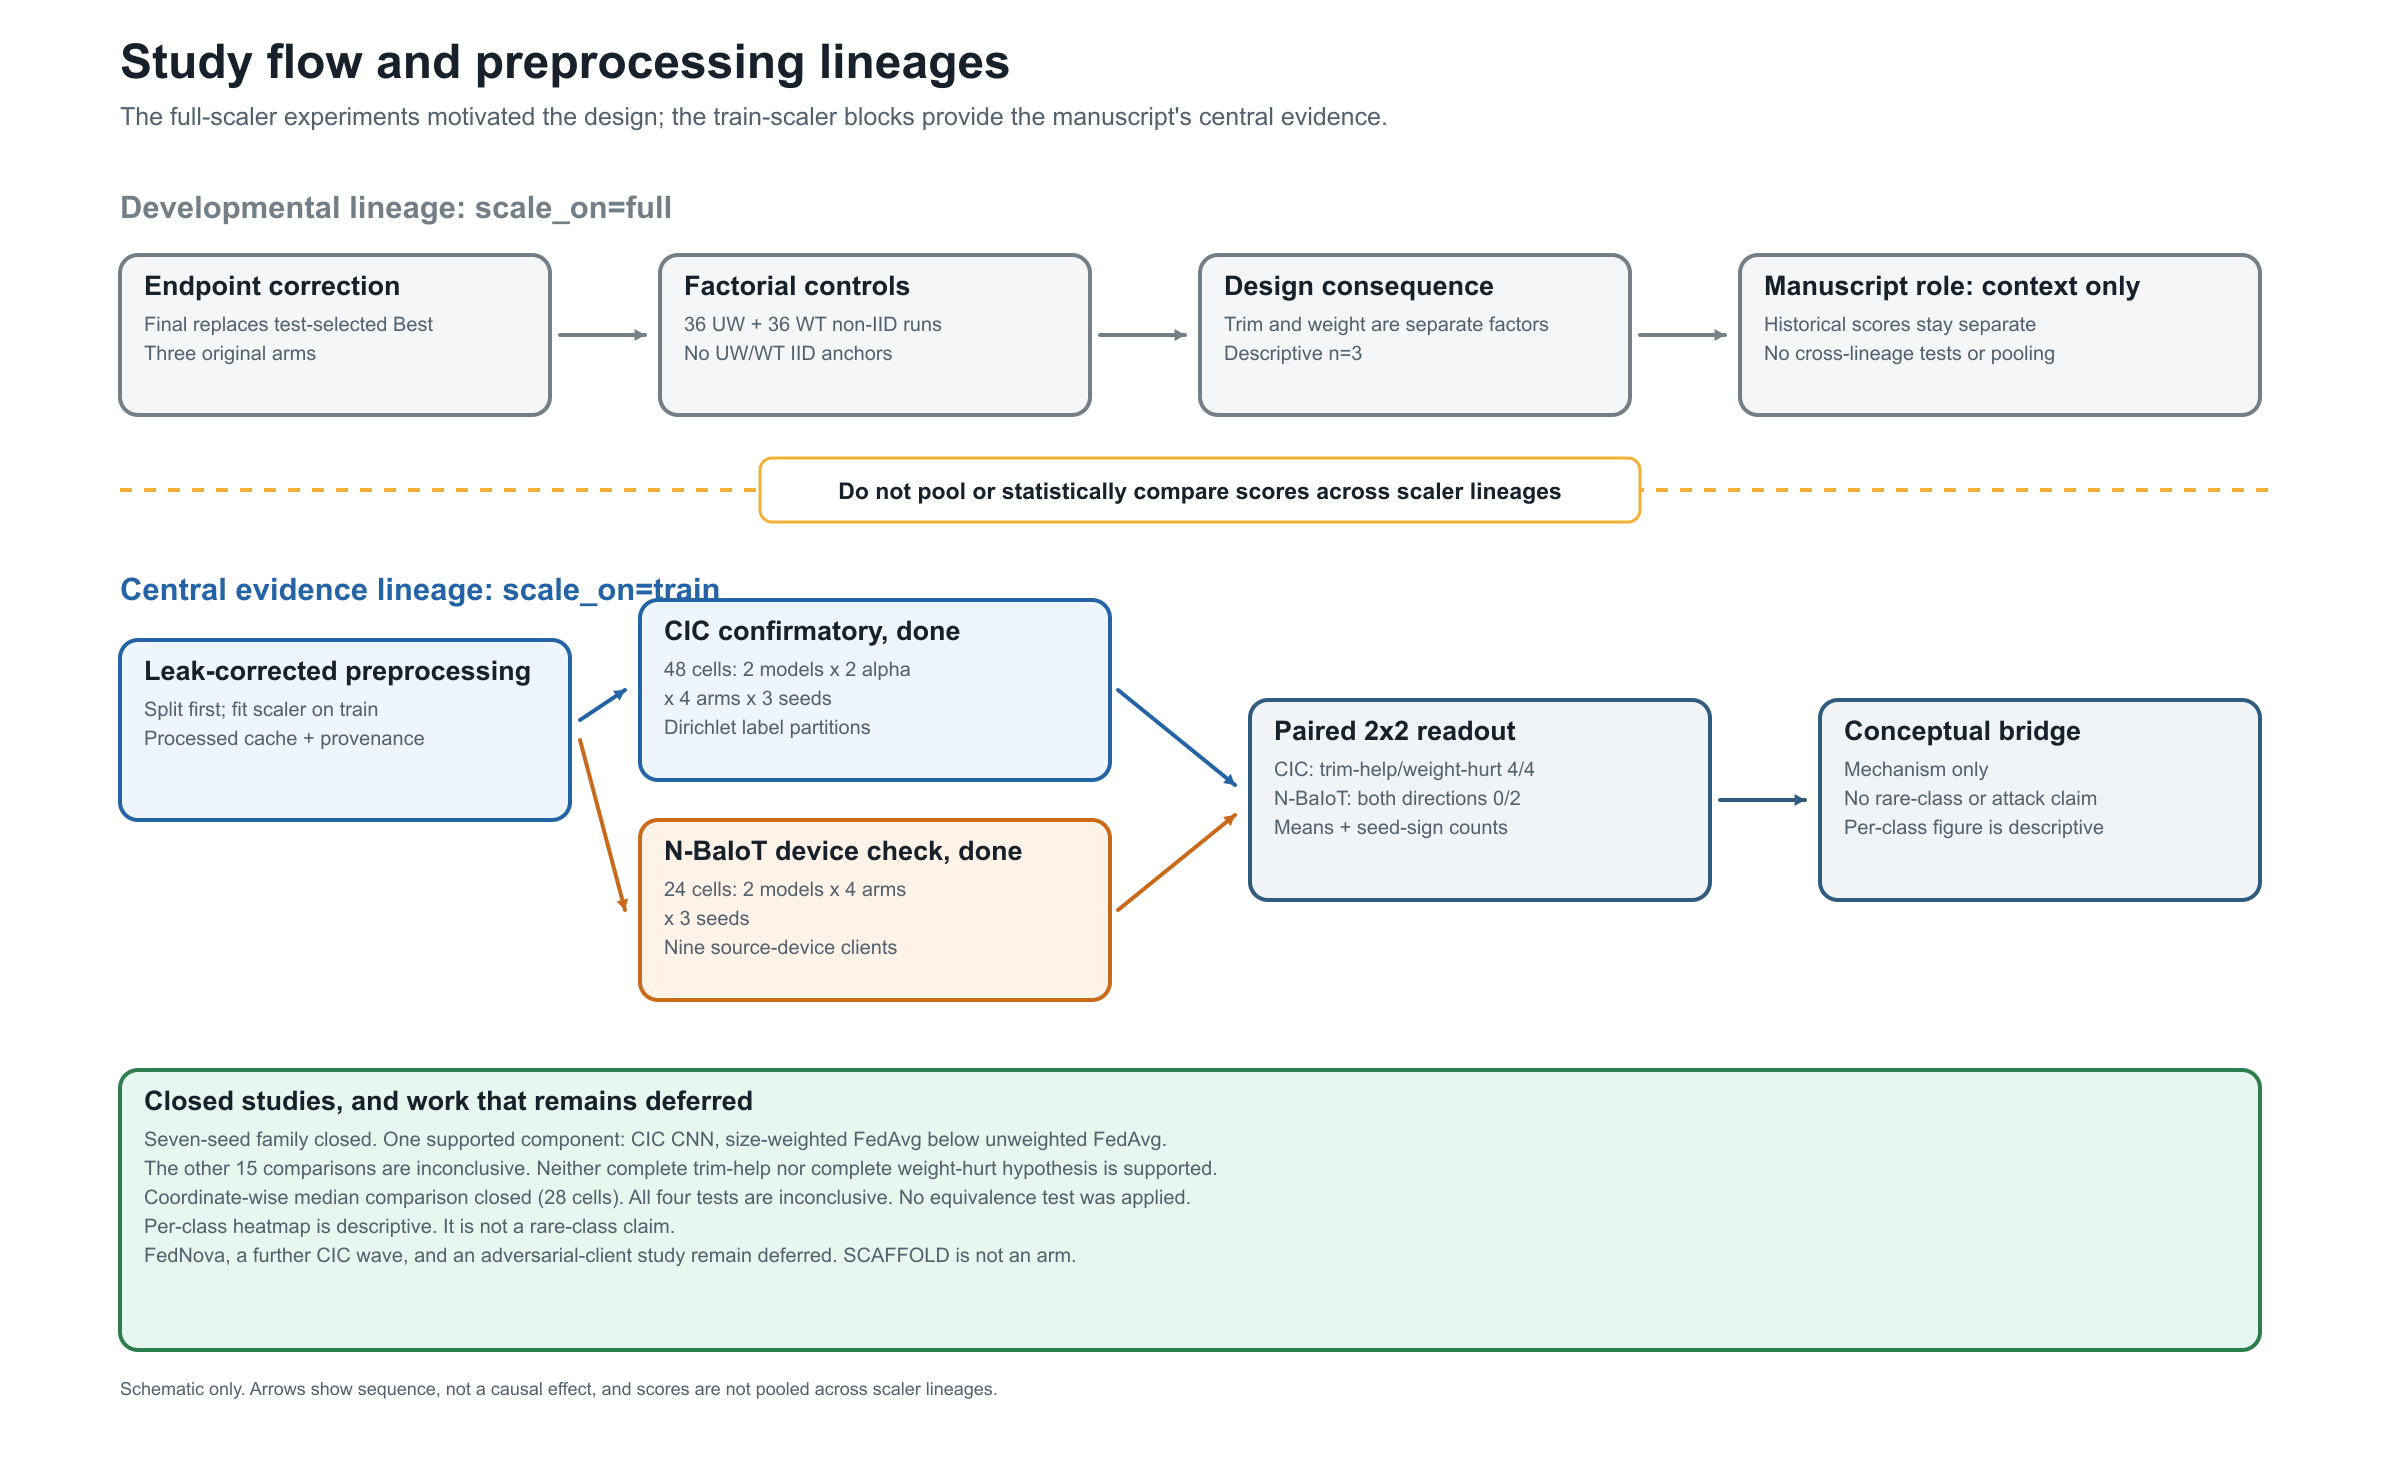
\includegraphics[width=\textwidth]{q1_study_lineages.png}
\caption{Study flow. Full-scaler experiments exposed the trim-versus-weight confound and stay in a separate lineage. Train-scaler blocks supply the central four-arm evidence. Arrows show sequence. Scores are not pooled across the two scaler lineages, and the figure is not a results table.}
\label{fig:lineages}
\end{figure*}

\section{Related work and scope}
FedAvg combines locally trained models using client-data-size weights \cite{mcmahan17}. FedProx modifies the local objective with a proximal term \cite{li20}; SCAFFOLD instead uses control variates to correct client drift \cite{karimireddy20}; and FedNova normalizes heterogeneous local progress to address objective inconsistency \cite{wang20fednova}. These methods intervene at different points in the optimization process. SCAFFOLD and FedNova are relevant heterogeneity-aware methods, but neither is an arm in the completed experiments below, and neither substitutes for the two-factor test of server-side trimming and client-size weighting.

Empirical work has shown that the type and degree of non-IID partitioning can materially change decentralized-learning accuracy \cite{hsieh20}, and a broad comparison found no single evaluated FL method best in every non-IID case \cite{li22noniid}. Label-distribution-skew methods such as FedLC explicitly target local minority and missing classes \cite{zhang22fedlc}. Those findings motivate class-wise measurement, but they do not establish that any rare class improved in our runs. Coordinate-wise trimmed means address a different problem: their Byzantine analyses allow arbitrary or adversarial worker behavior \cite{yin18}. A guarantee under that threat model cannot be transferred to honest device clients or to our trimmed-parameter implementation without checking its assumptions.

Recent Byzantine-robust work with label skew has examined the tension between heterogeneous honest gradients and defenses built around a majority of similar updates \cite{bao24}. The experiments below inject no malicious clients. They ask whether a fixed coordinate-wise trim changes class-balanced detection when all nine simulated clients follow the same training code, and whether client-size weighting changes that answer.

The coordinate-wise median is a different summary from the geometric median. Pillutla, Kakade, and Harchaoui aggregate client updates with a geometric median in order to limit corrupted updates \cite{pillutla22}. That aggregator is not used here. Cambus, Melnyk, Milentijevic, and Schmid study the coordinate-wise median under Byzantine clients \cite{cambus25}. With nine clients, the median in this article is the fifth ordered value on each coordinate, and clients are not weighted by sample size. Yin \emph{et al.} give statistical rates for both the coordinate-wise median and the coordinate-wise trimmed mean in a Byzantine model \cite{yin18}. Those rates are not a result about the honest clients below.

Client weights also come in more than one form. Nguyen, Wu, and Chang reweight individual samples so that a client's distribution moves toward a global distribution \cite{nguyen24weights}. Wilbik, P\k{e}kala, Dyczkowski, and Szko{\l}a compare client weights that depend on local model quality \cite{wilbik23}. The size weights in this article multiply an entire client parameter vector by that client's training-set size. Sample weights and quality weights are not arms.

Federated IoT anomaly and botnet detection has prior domain precedent \cite{nguyen19diot,popoola22}. The N-BaIoT and CIC-IoT2023 source studies establish the two traffic corpora \cite{meidan18,neto23}. Albanbay \emph{et al.} compare model families and local data volume for federated intrusion detection on CICIoT2023, including a convolutional network, under a simulated device population \cite{albanbay25}. Their question is model and data scale. The question here is the aggregation factorial on processed versions of CIC-IoT2023 and N-BaIoT.

Table~\ref{tab:closest} states what the controlled $2\times2$ adds. The table is a scope comparison. It is not a claim to be the first study of robust aggregation, client weighting, or federated IoT detection.

\begin{table*}[!t]
\centering
\caption{Closest related studies. Each row names the question that study asks. The last column is the increment from crossing coordinate-wise trimming with client-size weighting on the two processed corpora in this article.}
\label{tab:closest}
\small
\begin{tabular}{p{2.5cm}p{6.3cm}p{7.2cm}}
\hline
Study & Question in that study & Increment from this $2\times2$ \\
\hline
Yin \emph{et al.} \cite{yin18} & Byzantine rates for coordinate-wise median and trimmed mean & Honest clients only. Trimming is crossed with client-size weights. \\
Pillutla \emph{et al.} \cite{pillutla22} & Geometric median under corrupted updates & A different aggregator. The geometric median is not an arm. \\
Cambus \emph{et al.} \cite{cambus25} & Coordinate-wise median with Byzantine clients & Nine honest clients. The rule is the fifth ordered value. The comparison with the trimmed mean is a separate four-test family. \\
Nguyen \emph{et al.} \cite{nguyen24weights} & Sample weights for distribution skew & Weights here scale whole client vectors by training-set size. \\
Wilbik \emph{et al.} \cite{wilbik23} & Client weights from local model quality & Size weights are crossed with trimming. Quality weights are not an arm. \\
Bao \emph{et al.} \cite{bao24} & Byzantine robustness under label skew & No malicious client is injected. \\
Albanbay \emph{et al.} \cite{albanbay25} & Model and data scale for federated detection on CICIoT2023 & Aggregation factorial on processed CIC-IoT2023 and N-BaIoT. \\
D{\"I}oT and Popoola \emph{et al.} \cite{nguyen19diot,popoola22} & Federated IoT anomaly and botnet detection & Controlled aggregator comparison on two existing corpora. \\
\hline
\end{tabular}
\end{table*}

\section{Methods}
\subsection{Data, partitions, and preprocessing lineages}
N-BaIoT contains traffic from nine commercial IoT device identities \cite{meidan18}; the task here has 11 classes and 115 numeric features. CIC-IoT2023 contributes a separate eight-category task with 39 numeric flow features \cite{neto23}. Table~\ref{tab:data} summarizes the resulting processed caches. The experiments cap each source file at 20,000 rows. A stratified split with seed 42 produces pooled train and test sets. For the two blocks analyzed below, a StandardScaler is fit on the \emph{pooled training matrix only} and then applied to train and test. This avoids fitting the scaler on test records, but is not fully local or privacy-preserving preprocessing: the scaler uses pooled training data.

\begin{table*}[!t]
\centering
\caption{The two separate train-only-scaled experiment blocks. Counts refer to the processed, capped caches, not the original source datasets. Neither block tests deployment.}
\label{tab:data}
\small
\begin{tabular}{lcccccl}
\hline
Block & Train & Test & Features & Classes & Clients & Client construction \\
\hline
CIC-IoT2023 & 4,825,692 & 1,206,424 & 39 & 8 & 9 & Dirichlet label allocation \\
N-BaIoT & 1,418,112 & 354,529 & 115 & 11 & 9 & Source device identity \\
\hline
\end{tabular}
\end{table*}

The CIC confirmatory block partitions labels among nine simulated clients at $\alpha=0.5$ and $0.1$. It includes two architectures, four aggregation arms, and seeds $\{42,123,7\}$, giving 48 cells. Its separate $\alpha=1.0$ smoke run is not an additional ranking campaign. The N-BaIoT block assigns each train record to its source device identity, giving nine non-empty, disjoint clients and 24 model-by-arm-by-seed cells. Its pooled test split contains records from all nine identities. It therefore measures held-out records from \emph{participating} devices, not generalization to unseen devices. Seven N-BaIoT training clients contain all 11 classes; the Ennio doorbell and Samsung webcam each contain six and have no Mirai examples in this corpus. This observed coverage difference must not be mistaken for measured per-class performance.

The earlier full-scaler tables used \texttt{scale\_on=full}. They are retained as historical context but are not numerically combined with the \texttt{scale\_on=train} CIC and N-BaIoT tables in this manuscript. In particular, a change between the two tracks cannot be attributed to an aggregator without accounting for preprocessing and other design differences.

\subsection{Models and four aggregation arms}
The MLP has hidden widths 128, 64, 64, and 32 with ReLU activations and layer normalization; its first three hidden blocks use dropout rates 0.2, 0.2, and 0.1. The one-dimensional CNN treats each feature vector as a sequence, applies two convolutional layers (1-to-32 channels with kernel 5, then 32-to-64 with kernel 3), adaptive average pooling, and a 64-to-32-to-classifier head. These are the same implementations used across the four arms within each block, rather than new architectures tuned separately per aggregator. All clients participate in each of 30 communication rounds. Each client trains for three local epochs with Adam at learning rate $10^{-3}$ and batch size 512 before returning model parameters. The server evaluates the aggregated model on the pooled holdout after each round. The same architecture and seed are used within each four-arm comparison.

Table~\ref{tab:factorial} displays the factorial interpretation. Let $w_k$ denote a returned client parameter vector, $n_k$ its training-set size, and $n=\sum_{k=1}^{K}n_k$. The untrimmed arms are size-weighted FedAvg (FA) and unweighted FedAvg (UW):
\begin{equation}
w_{\mathrm{FA}}=\sum_{k=1}^{K}\frac{n_k}{n}w_k,\qquad
w_{\mathrm{UW}}=\frac{1}{K}\sum_{k=1}^{K}w_k.
\end{equation}
For each parameter coordinate, the trimmed arms sort the nine returned values and discard one value at each tail. FedTrimmedAvg (FT) averages the seven retained values equally; WeightedFedTrimmedAvg (WT) uses the retained clients' sample-size weights, normalized over those seven values. Thus the configured trimming fraction $0.1$ removes $1/9$ of the clients at each tail for this $K=9$ implementation. FedProx belongs to a separate, scoped optimizer/regularization investigation and is not a fifth arm of this factorial comparison.

More formally, let $S_j$ be the client indices retained for coordinate $j$ after removing the lowest and highest returned values. The two trimmed arms are
\begin{equation}
w_{\mathrm{FT},j}=\frac{1}{|S_j|}\sum_{k\in S_j}w_{k,j},\qquad
w_{\mathrm{WT},j}=\frac{\sum_{k\in S_j}n_k w_{k,j}}{\sum_{k\in S_j}n_k}.
\end{equation}
Because $S_j$ is coordinate-specific, WT is not obtained by selecting seven whole client models once per round; the survivor set can differ across parameters.

\begin{table}[!t]
\centering
\caption{The four aggregation arms as a two-factor design.}
\label{tab:factorial}
\small
\begin{tabular}{lcc}
\hline
Arm & Coordinate trim & Size weights \\
\hline
UW & No & No \\
FA & No & Yes \\
FT & Yes & No \\
WT & Yes & Yes \\
\hline
\end{tabular}
\end{table}

\subsection{Endpoints and prespecified directional rules}
The primary reported endpoints are Final accuracy, Final macro-F1, and the mean of round-wise macro-F1 across rounds 1--30. Best-round metrics are secondary diagnostics, never substitutes for Final. Macro-F1 is the arithmetic mean of the per-class F1 values, each formed from its class precision and recall. For each model and each CIC $\alpha$ cell, the preregistered contrasts are $\mathrm{FT}-\mathrm{UW}$ and $\mathrm{WT}-\mathrm{FA}$ for adding trimming, and $\mathrm{FA}-\mathrm{UW}$ and $\mathrm{WT}-\mathrm{FT}$ for adding size weighting. A trim-help direction requires \emph{both} mean trim contrasts to be positive; a weight-hurt direction requires \emph{both} mean weight contrasts to be negative. The N-BaIoT device block uses the same directional pair definitions by model. Its preregistration contains no FT-first ranking hypothesis. All three-seed directional results use unrounded, stored Final macro-F1 means over three matched seeds; exact ties do not meet the descriptive directional rule. The word ``supported'' is reserved for the seven-seed Holm decision. We report paired seed signs as well as means and make no $n=3$ significance or equivalence claim. The seven-seed family in Section~\ref{sec:e4} uses a different, preregistered rule: 16 two-sided paired $t$ tests on seeds $\{127,131,137,139,149,151,157\}$, with Holm correction across all 16 tests at $0.05$. That rule does not reclassify the three-seed tables.

\subsection{Integrity and reporting controls}
Each completed row is bound to the processed train-scaler cache and metadata hashes recorded for its experiment block. Histories contain exactly 30 rounds, and the stored Final macro-F1 is reconciled to round 30 before a cell counts as complete. The CIC and N-BaIoT manifests seal the current processed caches and written histories; they do not independently hash every original source CSV. Final accuracy and Final macro-F1 use round 30 and are not replaced by their maxima over 30 pooled-test evaluations. This prevents a test-selected best round from replacing the prespecified final model in the main comparison.

\section{Results}
\subsection{Train-only-scaled CIC-IoT2023 confirmatory block}
Table~\ref{tab:cic} gives three-seed means of all three primary endpoints. Under the prespecified Final macro-F1 scoring rule, FT has the highest arm mean, both trim contrasts have positive means, and both weight contrasts have negative means in each of the four model-by-$\alpha$ cells. This means the descriptive directional rule is met in all four cells, not that every individual seed has the same sign or that a significance test passed.

\begin{table*}[!t]
\centering
\caption{CIC-IoT2023 train-only-scaled confirmatory grid: three-seed means of the three primary endpoints. ``Round mean F1'' is the mean of 30 round-wise macro-F1 values, not ROC-AUC. FA, UW, FT, and WT are defined in Methods. Directional decisions use unrounded Final macro-F1, not the displayed five-decimal means.}
\label{tab:cic}
\small
\begin{tabular}{llcccc}
\hline
Model & $\alpha$ & Arm & Final Acc & Final F1 & Round mean F1 \\
\hline
MLP & 0.5 & FA & 0.88929 & 0.61594 & 0.59854 \\
    &     & UW & 0.89461 & 0.66156 & 0.64397 \\
    &     & FT & 0.89369 & 0.67497 & 0.65881 \\
    &     & WT & 0.89484 & 0.66704 & 0.65075 \\
MLP & 0.1 & FA & 0.85784 & 0.42598 & 0.42049 \\
    &     & UW & 0.83488 & 0.55188 & 0.53443 \\
    &     & FT & 0.83486 & 0.59686 & 0.58791 \\
    &     & WT & 0.82842 & 0.50295 & 0.48721 \\
CNN & 0.5 & FA & 0.88626 & 0.57053 & 0.53056 \\
    &     & UW & 0.89250 & 0.63050 & 0.58582 \\
    &     & FT & 0.89232 & 0.63993 & 0.59024 \\
    &     & WT & 0.89362 & 0.63511 & 0.58531 \\
CNN & 0.1 & FA & 0.85276 & 0.40552 & 0.38295 \\
    &     & UW & 0.86244 & 0.46235 & 0.43128 \\
    &     & FT & 0.83198 & 0.52651 & 0.46655 \\
    &     & WT & 0.78348 & 0.43521 & 0.37436 \\
\hline
\end{tabular}
\end{table*}

\subsection{Train-only-scaled N-BaIoT device block}
Table~\ref{tab:e2} reports the corresponding device-partition means for all three primary endpoints. Neither descriptive directional rule was met for either model: both N-BaIoT scores are $0/2$. FT minus UW is negative in all three seeds in both models, whereas WT minus FT is positive in all three seeds in both models. The remaining contrast signs vary by seed. WT has the highest descriptive MLP Final macro-F1 mean; UW exceeds WT by only about 0.22 percentage points in the CNN Final macro-F1 means. There is no preregistered FT-first decision for this block, and these rankings should not be treated as superiority or equivalence findings.

\begin{table*}[!t]
\centering
\caption{N-BaIoT nine-device partition: three-seed means of the three primary endpoints on a pooled holdout containing all nine device identities. ``Round mean F1'' is not ROC-AUC. This is not an unseen-device test.}
\label{tab:e2}
\small
\begin{tabular}{lcccc}
\hline
Model & Arm & Final Acc & Final F1 & Round mean F1 \\
\hline
MLP & FA & 0.82616 & 0.79348 & 0.76527 \\
    & UW & 0.81682 & 0.78192 & 0.75949 \\
    & FT & 0.81229 & 0.77297 & 0.76033 \\
    & WT & 0.83085 & 0.79982 & 0.76512 \\
CNN & FA & 0.80437 & 0.75374 & 0.73127 \\
    & UW & 0.81845 & 0.77796 & 0.72380 \\
    & FT & 0.79545 & 0.73851 & 0.73331 \\
    & WT & 0.81722 & 0.77580 & 0.72995 \\
\hline
\end{tabular}
\end{table*}

\subsection{Paired factor contrasts}
Table~\ref{tab:contrasts} exposes the paired Final macro-F1 contrasts used for the directional decisions. Values are mean percentage-point differences over the three matched seeds. Parentheses give the number of seeds with the prespecified direction: positive for the two trim contrasts and negative for the two weight contrasts. The CIC descriptive rule uses the signs of the unrounded three-seed means; the table makes clear where an individual seed disagrees. On N-BaIoT, neither descriptive directional rule was met.

\begin{table*}[!t]
\centering
\caption{Paired Final macro-F1 contrasts in percentage points, with desired-direction seed counts in parentheses. Required directions are $+$ for FT$-$UW and WT$-$FA, and $-$ for FA$-$UW and WT$-$FT.}
\label{tab:contrasts}
\small
\begin{tabular}{llcccc}
\hline
Block & Cell & FT$-$UW $(+)$ & WT$-$FA $(+)$ & FA$-$UW $(-)$ & WT$-$FT $(-)$ \\
\hline
CIC & MLP, $\alpha=0.5$ & +1.3405 (3/3) & +5.1101 (3/3) & $-$4.5623 (3/3) & $-$0.7927 (3/3) \\
CIC & MLP, $\alpha=0.1$ & +4.4978 (3/3) & +7.6971 (2/3) & $-$12.5899 (3/3) & $-$9.3906 (3/3) \\
CIC & CNN, $\alpha=0.5$ & +0.9438 (2/3) & +6.4580 (3/3) & $-$5.9970 (3/3) & $-$0.4828 (2/3) \\
CIC & CNN, $\alpha=0.1$ & +6.4167 (3/3) & +2.9693 (2/3) & $-$5.6830 (3/3) & $-$9.1304 (3/3) \\
N-BaIoT & MLP, device & $-$0.8952 (0/3) & +0.6333 (2/3) & +1.1559 (1/3) & +2.6844 (0/3) \\
N-BaIoT & CNN, device & $-$3.9444 (0/3) & +2.2054 (2/3) & $-$2.4216 (2/3) & +3.7283 (0/3) \\
\hline
\end{tabular}
\end{table*}

Figure~\ref{fig:paired} complements Table~\ref{tab:contrasts} by displaying every seed-level paired difference as well as its three-seed mean. It prevents a positive mean from being mistaken for unanimous agreement across the three seeds and makes the cross-setting sign reversal visible without combining raw performance levels.

\begin{figure*}[!t]
\centering
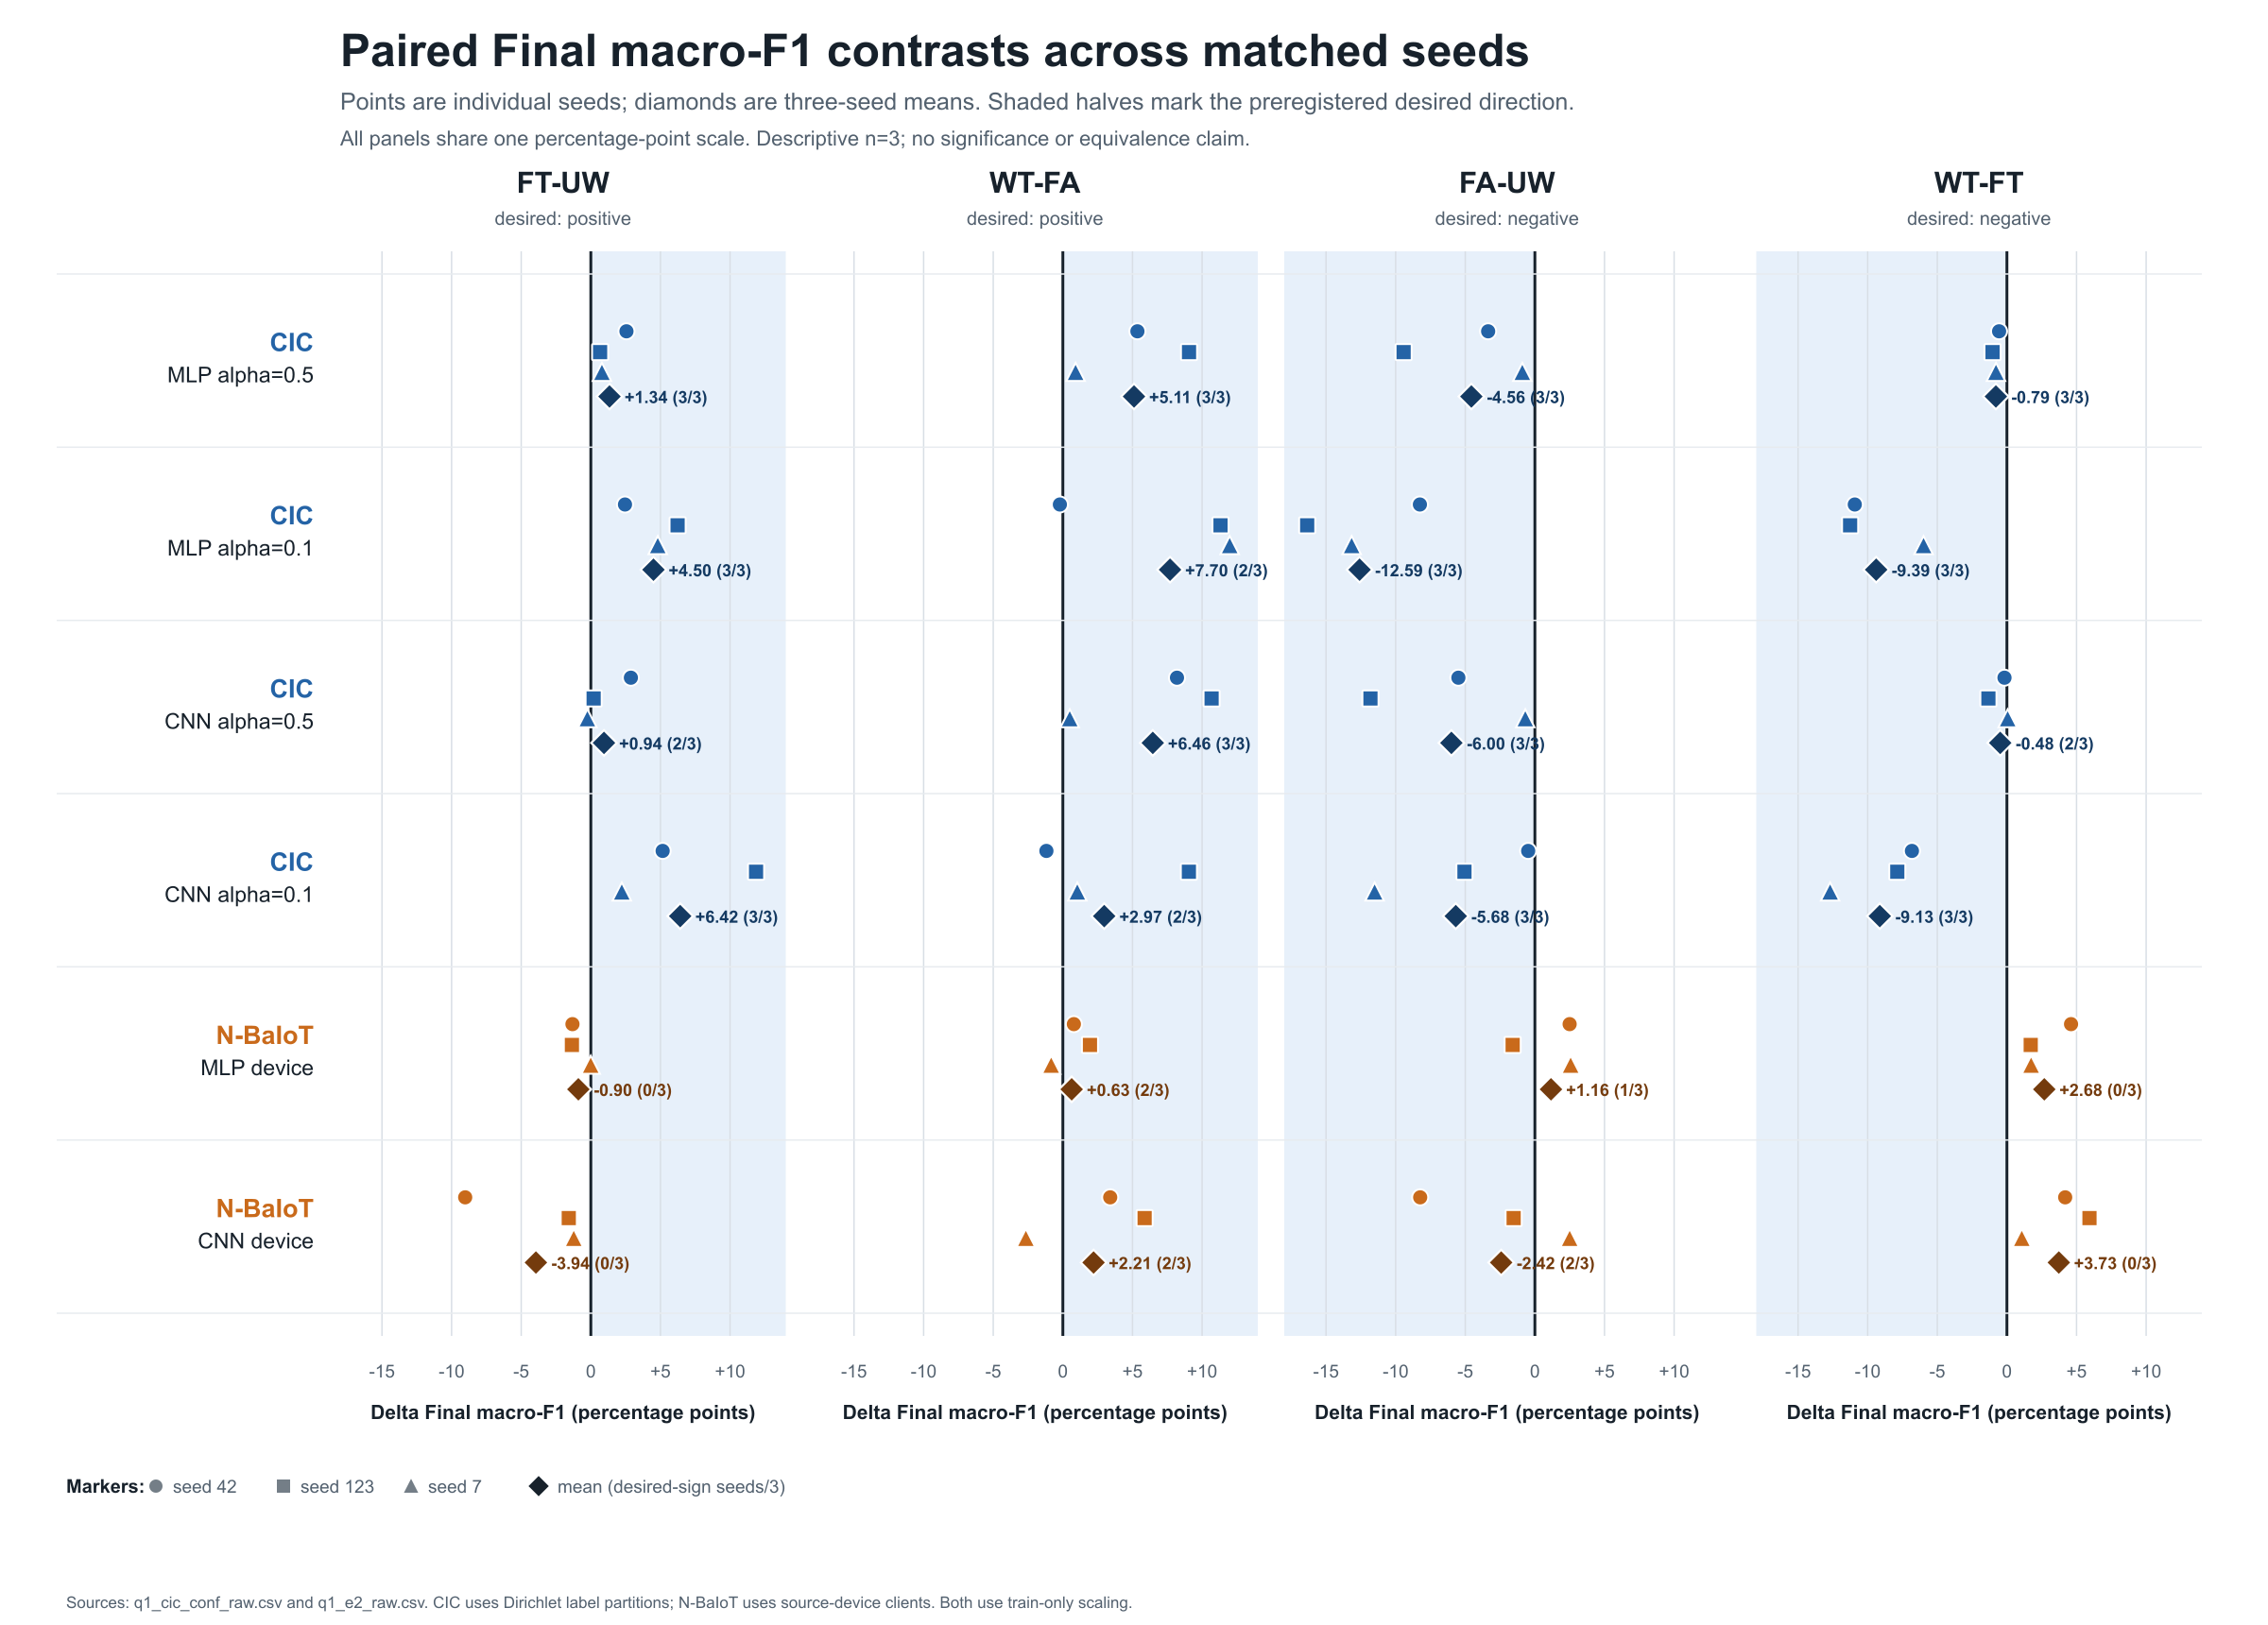
\includegraphics[width=\textwidth]{q1_paired_seed_contrasts.png}
\caption{Seed-level paired Final macro-F1 contrasts for the two trim and two weight comparisons. Small markers are the three matched seeds and diamonds are their means; the lightly shaded half of each panel is the prespecified desired direction. Counts report seeds in that direction. CIC and N-BaIoT are displayed together for sign-pattern comparison only; their scores are not pooled. All summaries are descriptive at $n=3$.}
\label{fig:paired}
\end{figure*}

The CIC and N-BaIoT directional outcomes differ, but the datasets and client partitions also differ. Their contrast signs can be discussed side by side; their raw scores are not pooled, and this study cannot isolate device partitioning as the cause of the difference. The 30-round histories also show that some CNN cells end substantially below their own best round. We therefore preserve the prespecified Final endpoint and report Best only as a secondary trajectory diagnostic.

\subsection{Seven-seed prospective family}
\label{sec:e4}
The three-seed boards above do not include a multiplicity-controlled test. That test was preregistered separately and is now closed. It uses the same train-only scaler, nine simulated clients, 30 rounds, and four arms, but only four blocks: CIC-IoT2023 MLP and CNN at Dirichlet $\alpha=0.1$ (T1 and T2), and the fixed N-BaIoT nine-device partition for MLP and CNN (T5 and T6). The CIC $\alpha=0.5$ cells are not in this family. On CIC, each new seed sets matched random conditions for all four arms. On N-BaIoT, the device partition stays fixed across seeds. The seven prospective seeds are $\{127,131,137,139,149,151,157\}$. The three earlier seeds are excluded from the tests. One hundred twelve new cells were completed. The endpoint is unrounded Final macro-F1 at round 30.

The family contains 16 two-sided paired comparisons: $\mathrm{FT}-\mathrm{UW}$ and $\mathrm{WT}-\mathrm{FA}$ for trimming, and $\mathrm{FA}-\mathrm{UW}$ and $\mathrm{WT}-\mathrm{FT}$ for size weighting, in each of the four blocks. Holm adjustment is across all 16 comparisons. A trim-help block is supported only when both trim comparisons are significant in the positive direction. A weight-hurt block is supported only when both weight comparisons are significant in the negative direction. Any other significant direction is a reversal for that comparison. Otherwise the comparison is inconclusive. Inconclusive does not mean the arms are equivalent, and no equivalence test was run.

Table~\ref{tab:e4} reports every comparison. Means and intervals are shown to four decimal places, and $p$-values use up to six significant digits. Only one comparison meets the decision rule. On T2, the CIC CNN, $\mathrm{FA}-\mathrm{UW}$ has mean $-10.7252$ percentage points, unadjusted 95\% paired-$t$ interval $[-15.9527,-5.4977]$, signs $0/0/7$, raw $p=0.00240333$, and Holm-adjusted $p=0.0384533$. Size weighting is associated with a lower Final macro-F1 than equal client weights in that one block. The other 15 comparisons are inconclusive. There is no reversal.

\begin{table*}[!t]
\centering
\caption{Seven-seed family, Question~1. Paired Final macro-F1 differences, in percentage points. The interval is the unadjusted 95\% paired-$t$ confidence interval. Signs are positive, tie, and negative counts. Holm adjustment uses all 16 rows. Only T2 $\mathrm{FA}-\mathrm{UW}$ is supported. This paired-$t$ Holm family is the preregistered decision.}
\label{tab:e4}
\scriptsize
\begin{tabular}{llrrrrlr}
\hline
Block & Contrast & Mean & 95\% CI & Signs & Raw $p$ & Holm $p$ & Decision \\
\hline
T1 & FT$-$UW & 0.3714 & $[-4.2080,\ 4.9507]$ & 5/0/2 & 0.849257 & 1 & inconclusive \\
T1 & WT$-$FA & 7.4325 & $[2.6661,\ 12.1990]$ & 7/0/0 & 0.00880574 & 0.12328 & inconclusive \\
T1 & FA$-$UW & $-12.2101$ & $[-19.7262,\ -4.6941]$ & 1/0/6 & 0.00732394 & 0.109859 & inconclusive \\
T1 & WT$-$FT & $-5.1490$ & $[-13.1925,\ 2.8946]$ & 2/0/5 & 0.168306 & 1 & inconclusive \\
T2 & FT$-$UW & $-1.5393$ & $[-4.7906,\ 1.7121]$ & 3/0/4 & 0.290708 & 1 & inconclusive \\
T2 & WT$-$FA & 6.3105 & $[1.1477,\ 11.4734]$ & 6/0/1 & 0.024293 & 0.315809 & inconclusive \\
T2 & FA$-$UW & $-10.7252$ & $[-15.9527,\ -5.4977]$ & 0/0/7 & 0.00240333 & 0.0384533 & supported \\
T2 & WT$-$FT & $-2.8754$ & $[-7.8214,\ 2.0706]$ & 2/0/5 & 0.20472 & 1 & inconclusive \\
T5 & FT$-$UW & $-0.0201$ & $[-2.4796,\ 2.4394]$ & 4/0/3 & 0.984693 & 1 & inconclusive \\
T5 & WT$-$FA & $-1.7038$ & $[-3.2609,\ -0.1466]$ & 0/0/7 & 0.0366684 & 0.440021 & inconclusive \\
T5 & FA$-$UW & 1.6414 & $[-0.7365,\ 4.0193]$ & 5/0/2 & 0.142178 & 1 & inconclusive \\
T5 & WT$-$FT & $-0.0423$ & $[-1.3127,\ 1.2281]$ & 4/0/3 & 0.937724 & 1 & inconclusive \\
T6 & FT$-$UW & 0.7091 & $[-3.2827,\ 4.7008]$ & 6/0/1 & 0.679 & 1 & inconclusive \\
T6 & WT$-$FA & 1.2596 & $[-4.7011,\ 7.2203]$ & 2/0/5 & 0.623612 & 1 & inconclusive \\
T6 & FA$-$UW & $-0.4904$ & $[-5.7321,\ 4.7514]$ & 3/0/4 & 0.826545 & 1 & inconclusive \\
T6 & WT$-$FT & 0.0601 & $[-4.2701,\ 4.3904]$ & 2/0/5 & 0.974004 & 1 & inconclusive \\
\hline
\end{tabular}
\end{table*}

Neither complete hypothesis is supported. Trim-help requires both trim comparisons in a block to be supported in the positive direction, and no block meets that requirement. Weight-hurt requires both weight comparisons in a block to be supported in the negative direction, and no block meets that requirement. The supported T2 $\mathrm{FA}-\mathrm{UW}$ result is one of the two weight components in that block. T2 $\mathrm{WT}-\mathrm{FT}$ is inconclusive, with Holm-adjusted $p=1$. Ten-seed summaries were prespecified as descriptive and are not used to override Table~\ref{tab:e4}.

\begin{figure*}[!t]
\centering
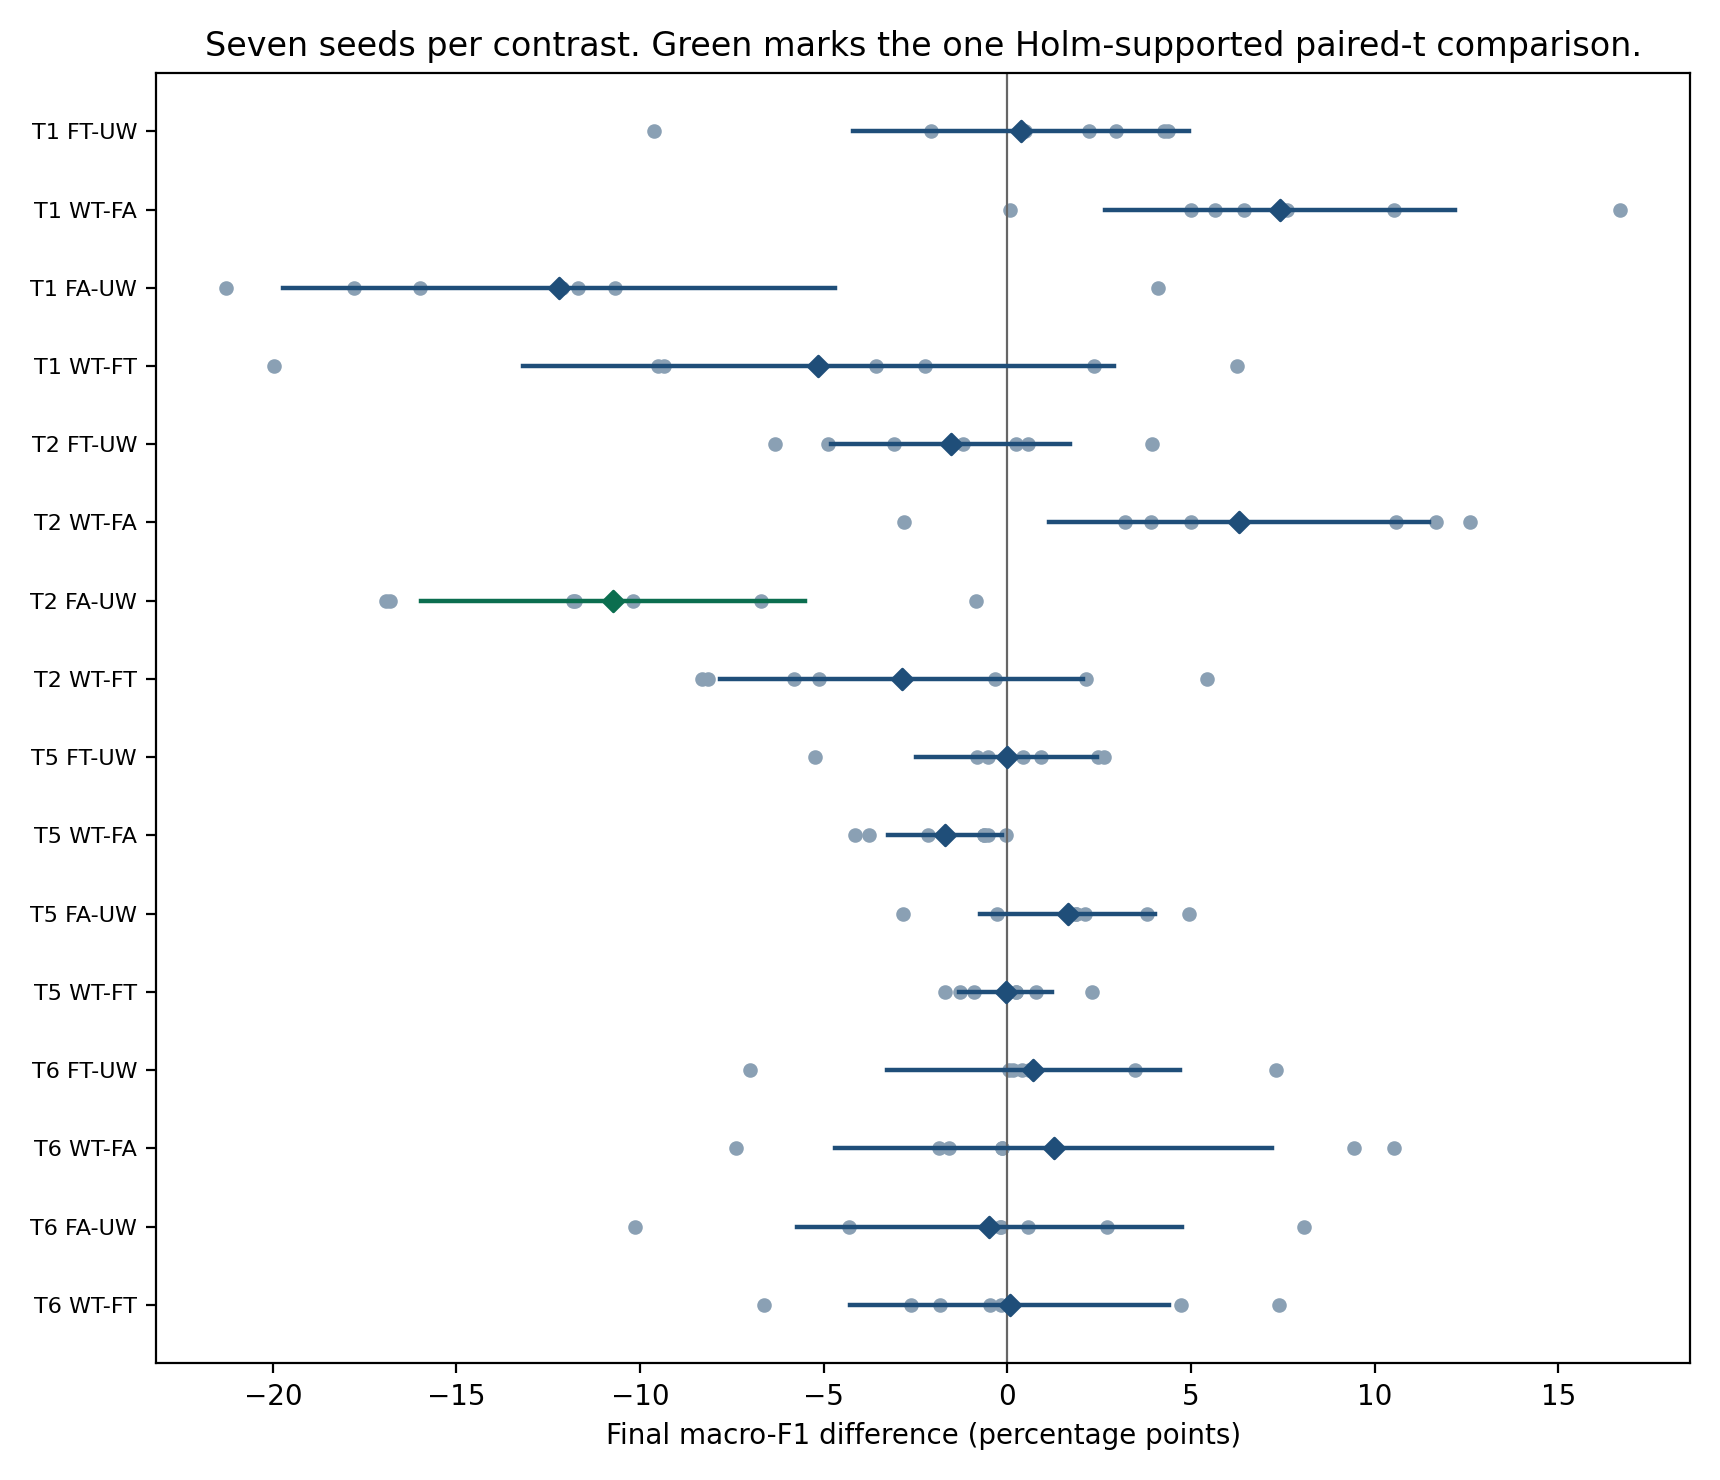
\includegraphics[width=\textwidth]{generated/q1_e4_forest.png}
\caption{All 16 seven-seed contrasts. Dots are the seven paired Final macro-F1 differences, in percentage points. The bar is the unadjusted 95\% paired-$t$ interval and the diamond is the mean. The green row is the one comparison with paired-$t$ Holm-adjusted $p<0.05$.}
\label{fig:forest}
\end{figure*}

\subsection{Exact sign-flip sensitivity}
The paired-$t$ test at $n=7$ leans on a normal approximation for the mean of seven differences. A post-hoc exact sign-flip test uses the same seven differences and makes a weaker assumption: under exchangeability of the sign of each paired difference, all $2^{7}=128$ sign assignments are equally likely. The statistic is the absolute sum of the signed differences. The two-sided $p$-value is the fraction of the 128 assignments whose absolute sum is at least the observed absolute sum. Holm adjustment is then applied to these 16 exact $p$-values.

Table~\ref{tab:signflip} reports that sensitivity. No comparison has a sign-flip Holm-adjusted $p$-value below $0.25$. The smallest raw values are $2/128=0.015625$, for T1 $\mathrm{WT}-\mathrm{FA}$, T2 $\mathrm{FA}-\mathrm{UW}$, and T5 $\mathrm{WT}-\mathrm{FA}$. With seven nonzero differences, $2/128$ is the smallest two-sided $p$-value this enumeration can return. Holm adjustment across 16 tests therefore cannot fall below $16\times 2/128=0.25$. The exact family-wise test cannot resolve this 16-comparison family at level $0.05$ when each contrast has only seven seeds. The preregistered paired-$t$ Holm decision remains the official result, and under that rule T2 $\mathrm{FA}-\mathrm{UW}$ stays supported. Reviewers should see both statements together: the official test supports one weighting contrast, and the small-sample exact test supports none.

\begin{table}[!t]
\centering
\caption{Post-hoc exact sign-flip $p$-values for the 16 contrasts in Table~\ref{tab:e4}. Holm adjustment uses these 16 exact $p$-values only. No row is supported at $0.05$. This table is a sensitivity analysis, not a replacement for Table~\ref{tab:e4}.}
\label{tab:signflip}
\scriptsize
\begin{tabular}{llrr}
\hline
Block & Contrast & Sign-flip $p$ & Holm $p$ \\
\hline
T1 & FT$-$UW & 0.875000 & 1 \\
T1 & WT$-$FA & 0.015625 & 0.250000 \\
T1 & FA$-$UW & 0.031250 & 0.406250 \\
T1 & WT$-$FT & 0.171875 & 1 \\
T2 & FT$-$UW & 0.281250 & 1 \\
T2 & WT$-$FA & 0.031250 & 0.406250 \\
T2 & FA$-$UW & 0.015625 & 0.250000 \\
T2 & WT$-$FT & 0.187500 & 1 \\
T5 & FT$-$UW & 0.968750 & 1 \\
T5 & WT$-$FA & 0.015625 & 0.250000 \\
T5 & FA$-$UW & 0.156250 & 1 \\
T5 & WT$-$FT & 0.937500 & 1 \\
T6 & FT$-$UW & 0.515625 & 1 \\
T6 & WT$-$FA & 0.640625 & 1 \\
T6 & FA$-$UW & 0.828125 & 1 \\
T6 & WT$-$FT & 0.968750 & 1 \\
\hline
\end{tabular}
\end{table}

\subsection{Trimming-by-weighting interaction}
The interaction $(\mathrm{WT}-\mathrm{FA})-(\mathrm{FT}-\mathrm{UW})$ was prespecified as a descriptive summary. It is outside the 16-test Holm family, and no interaction $p$-value is used as a decision. Table~\ref{tab:interaction} and Fig.~\ref{fig:interaction} report the seven-seed mean, the unadjusted 95\% paired-$t$ interval, and the positive, tie, and negative seed counts. On T1 and T2 the interval excludes zero. On T5 and T6 it includes zero. These intervals describe the estimates. They do not add a fifth supported comparison, and they do not change Table~\ref{tab:e4}.

\begin{table}[!t]
\centering
\caption{Descriptive trimming-by-weighting interaction on the seven prospective seeds, in Final macro-F1 percentage points. Signs are positive, tie, and negative counts. No decision $p$-value is attached.}
\label{tab:interaction}
\small
\begin{tabular}{lrrl}
\hline
Block & Mean & 95\% interval & Signs \\
\hline
T1 & 7.0612 & $[0.3531,\ 13.7692]$ & 7/0/0 \\
T2 & 7.8498 & $[1.8981,\ 13.8015]$ & 6/0/1 \\
T5 & $-1.6837$ & $[-4.7734,\ 1.4060]$ & 3/0/4 \\
T6 & 0.5505 & $[-8.9670,\ 10.0680]$ & 2/0/5 \\
\hline
\end{tabular}
\end{table}

\begin{figure}[!t]
\centering
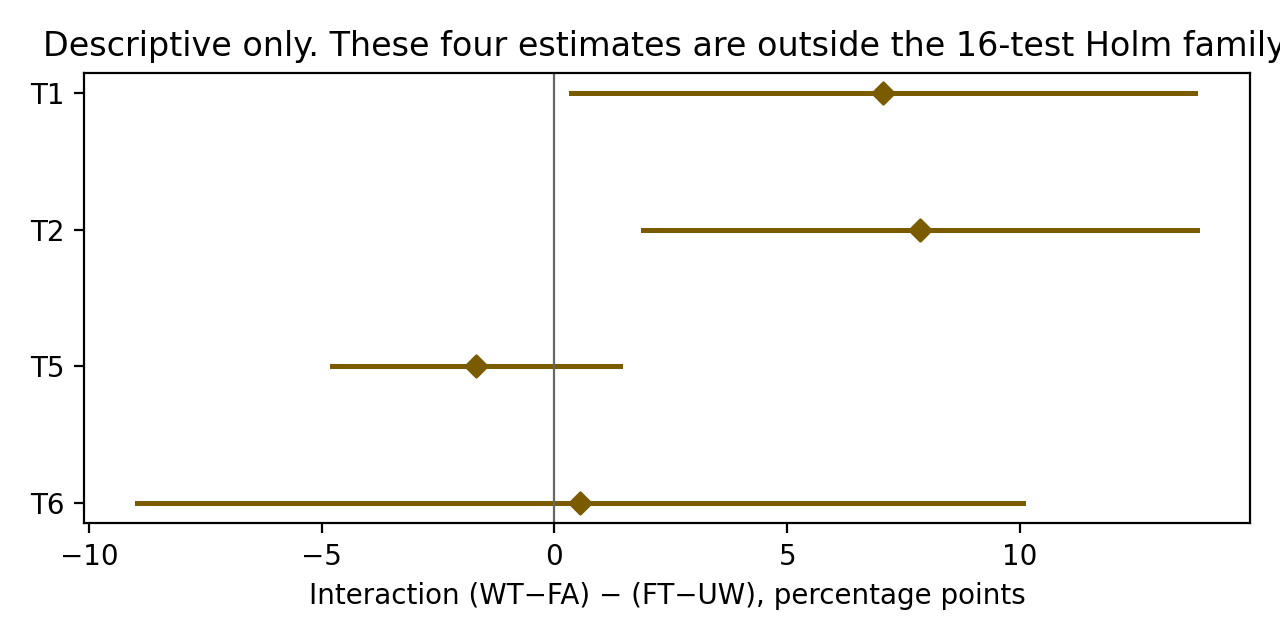
\includegraphics[width=\columnwidth]{generated/q1_e4_interaction.png}
\caption{Descriptive interaction estimates. The bar is the unadjusted 95\% paired-$t$ interval. These four estimates are outside the Holm family.}
\label{fig:interaction}
\end{figure}

\subsection{Coordinate-wise median comparison}
\label{sec:e5}
Question~3 is separate from Question~1. It asks whether the coordinate-wise trimmed mean differs from the coordinate-wise median. The comparison uses the same four blocks and the same seven seeds, $\{127,131,137,139,149,151,157\}$. Each median cell uses Adam at learning rate $10^{-3}$, three local epochs, batch size 512, and 30 rounds. On each coordinate the server keeps the fifth ordered value across the nine client updates and does not weight clients by sample size. The comparator is the trimmed-mean cell from the seven-seed family for the same block and seed. Those trimmed-mean cells were not retrained. FedNova is not an arm in this comparison. The supplement records why an earlier plan that included FedNova ended before any decision cell.

The endpoint is unrounded Final macro-F1 at round 30. Each test is a two-sided paired $t$ test on the seven seed-wise differences, trimmed mean minus coordinate-wise median, with $n=7$ and $\mathrm{df}=6$. Holm adjustment covers these four tests only, in the order T1, T2, T5, T6, at family-wise level $0.05$. A positive supported mean would say the trimmed mean is higher than the median in that block only. A negative supported mean would say the median is higher in that block only. This adjustment is not combined with Table~\ref{tab:e4}.

Table~\ref{tab:e5} reports every comparison. Means and intervals are in percentage points to four decimal places, and $p$-values use up to six significant digits. None of the four tests is supported. No equivalence procedure was applied, so the table does not establish that the trimmed mean and the median are interchangeable. The supported T2 $\mathrm{FA}-\mathrm{UW}$ result in Table~\ref{tab:e4} is unchanged.

\begin{table*}[!t]
\centering
\caption{Question~3. Paired Final macro-F1 differences, in percentage points, over seven seeds. The difference is the trimmed mean minus the coordinate-wise median. The interval is the unadjusted 95\% paired-$t$ confidence interval. Signs are negative, tie, and positive counts, in that order. Holm adjustment uses these four rows only. No row is supported.}
\label{tab:e5}
\scriptsize
\begin{tabular}{llrrrrlr}
\hline
Block & Contrast & Mean & 95\% CI & $-$/0/$+$ & Raw $p$ & Holm $p$ & Decision \\
\hline
T1 & FT$-$median & 0.3471 & $[-1.6900,\ 2.3842]$ & 3/0/4 & 0.691258 & 1 & inconclusive \\
T2 & FT$-$median & 0.6388 & $[-1.7203,\ 2.9980]$ & 3/0/4 & 0.532201 & 1 & inconclusive \\
T5 & FT$-$median & $-1.7913$ & $[-4.5363,\ 0.9537]$ & 4/0/3 & 0.161432 & 0.645727 & inconclusive \\
T6 & FT$-$median & $-1.6825$ & $[-4.8882,\ 1.5233]$ & 3/0/4 & 0.246421 & 0.739263 & inconclusive \\
\hline
\end{tabular}
\end{table*}

\subsection{Client heterogeneity}
Question~2 compares directional patterns, not raw scores. The two client constructions are also different in size and in label mix, and those differences can be measured without a new training run. Table~\ref{tab:hetero} uses the same Dirichlet allocations and the same device partition as the seven-seed family. A partition is included only when its hash matches the recorded configuration. Jensen--Shannon divergence is computed in bits between each client's training-label distribution and the pooled training-label distribution. A missing class is a class with zero training rows on that client.

On CIC-IoT2023 at $\alpha=0.1$, client size is highly unbalanced. The largest-to-smallest client ratio runs from $10.8$ to $1{,}555$, the coefficient of variation from $0.73$ to $1.63$, and the largest client's share of training rows from $0.270$ to $0.584$. Mean Jensen--Shannon divergence is between $0.357$ and $0.498$ bits. Every seed leaves at least one class missing from at least one client; the mean number of missing classes per client is about $1.22$ to $1.33$, and the worst client in a seed misses $2$ to $4$ classes.

The N-BaIoT device partition is much closer to balance. Its nine sizes run from $95{,}875$ to $176{,}174$ rows, so the largest-to-smallest ratio is $1.84$, the coefficient of variation is $0.209$, and the largest share is $0.124$. Mean Jensen--Shannon divergence is $0.054$ bits and the maximum is $0.233$ bits. The mean number of missing classes is $1.11$, while the worst client misses $5$ classes. That worst-client count is consistent with the two devices, the Ennio doorbell and the Samsung webcam, that contain six of the eleven classes and have no Mirai examples in this corpus.

These rows describe the partitions. They do not identify which change, dataset or client construction, produced the difference in directional pattern between CIC-IoT2023 and N-BaIoT.

\begin{table*}[!t]
\centering
\caption{Client-size imbalance, missing-class coverage, and label divergence for the seven-seed partitions. CIC rows are Dirichlet $\alpha=0.1$. The N-BaIoT row is the fixed device partition. JS is Jensen--Shannon divergence in bits against the pooled training-label distribution. Counts are rounded from the recomputed partition tables.}
\label{tab:hetero}
\scriptsize
\begin{tabular}{lrrrrrrrrr}
\hline
Partition & Min & Max & Max/min & CV & Largest share & Mean missing & Max missing & Mean JS & Max JS \\
\hline
CIC, seed 127 & 7,652 & 2,395,227 & 313.0 & 1.39 & 0.496 & 1.22 & 2 & 0.495 & 0.804 \\
CIC, seed 131 & 120,178 & 1,301,733 & 10.8 & 0.73 & 0.270 & 1.22 & 3 & 0.357 & 0.685 \\
CIC, seed 137 & 1,219 & 1,895,895 & 1,555.3 & 1.09 & 0.393 & 1.33 & 3 & 0.401 & 0.906 \\
CIC, seed 139 & 27,236 & 2,568,302 & 94.3 & 1.41 & 0.532 & 1.22 & 3 & 0.412 & 0.806 \\
CIC, seed 149 & 34,483 & 1,406,112 & 40.8 & 1.10 & 0.291 & 1.22 & 3 & 0.498 & 0.746 \\
CIC, seed 151 & 5,335 & 2,008,503 & 376.5 & 1.20 & 0.416 & 1.22 & 4 & 0.433 & 0.767 \\
CIC, seed 157 & 3,147 & 2,819,296 & 895.9 & 1.63 & 0.584 & 1.22 & 3 & 0.481 & 0.913 \\
N-BaIoT, device & 95,875 & 176,174 & 1.84 & 0.21 & 0.124 & 1.11 & 5 & 0.054 & 0.233 \\
\hline
\end{tabular}
\end{table*}

\subsection{Duplicate rows and source overlap}
Both datasets reuse a pooled train/test structure. The leakage check compares stored float32 feature rows by exact equality, which is the matrix the models saw. It does not rebuild the caches. A feature with zero variance can make distinct raw rows identical after scaling, so an exact match is evidence about the stored matrix, not a reconstructed raw-file identity.

The CIC training matrix has $4{,}825{,}692$ rows and $3{,}565{,}650$ unique rows. Of $1{,}206{,}424$ test rows, $381{,}765$ ($31.64\%$) are exact copies of some training row. All eight classes appear in both splits. The stored cache has no test source identifier, and the stored training source identifier takes only one value, so overlap of CIC source files between train and test cannot be counted from this cache.

The N-BaIoT training matrix has $1{,}418{,}112$ rows and $742{,}236$ unique rows. Of $354{,}529$ test rows, $211{,}718$ ($59.72\%$) are exact copies of some training row. All eleven classes appear in both splits. Source identifiers $0$ through $8$ appear in both splits, and all $354{,}529$ test rows come from a source that also appears in training. The N-BaIoT evaluation is a pooled within-device holdout. It is not a test on unseen devices.

\subsection{Per-class means on the three-seed CIC grid}
Fig.~\ref{fig:heatmap} shows mean per-class F1 for the CIC-IoT2023 MLP and CNN at $\alpha=0.1$, using the three seeds $\{42,123,7\}$ and all four arms. This display is descriptive. It is not part of the seven-seed Holm family, and it is not a rare-class finding. Mirai is near the top of the color scale for every arm on both models. Web remains low for every arm on both models. The figure shows that macro-F1 averages classes with very different detection levels. It does not identify which coordinates were trimmed.

\begin{figure*}[!t]
\centering
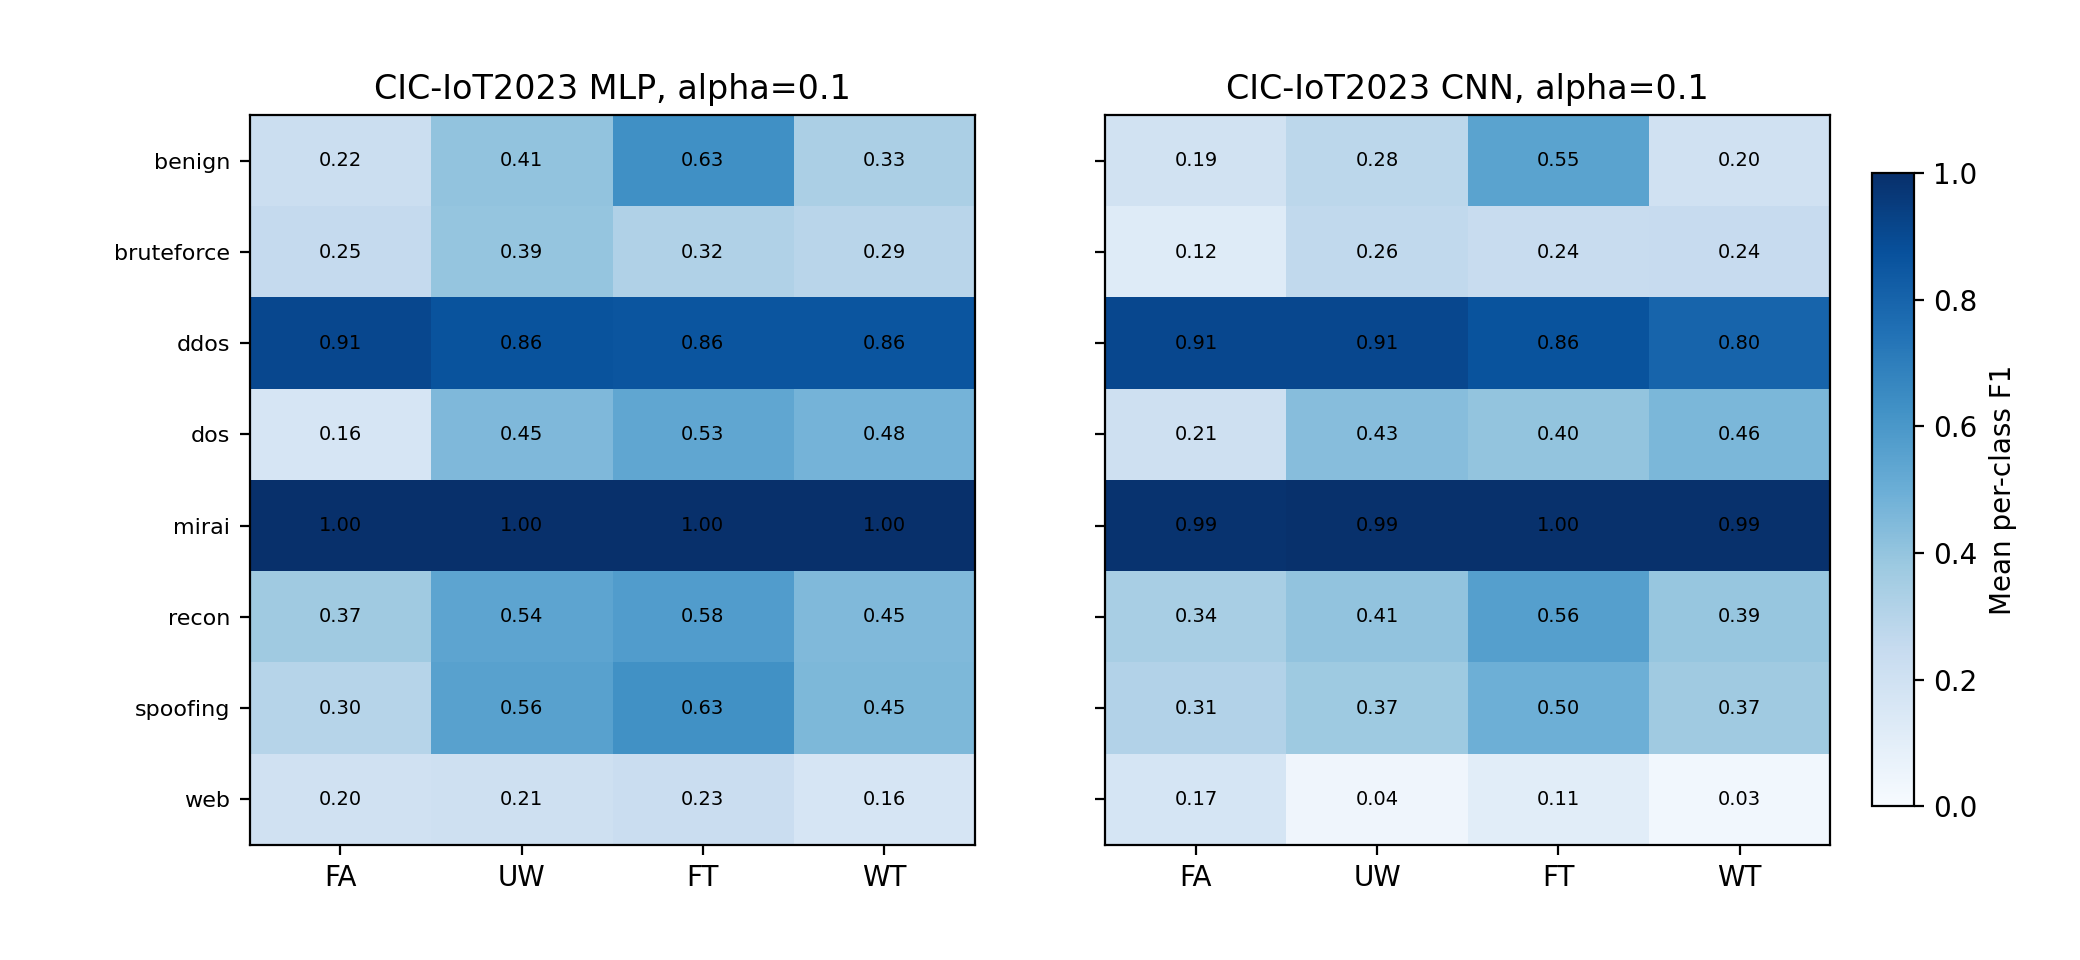
\includegraphics[width=\textwidth]{generated/q1_e7_heatmap.png}
\caption{Three-seed mean per-class F1 on CIC-IoT2023 at $\alpha=0.1$. Columns are the four arms. The display is descriptive and is not a Holm test.}
\label{fig:heatmap}
\end{figure*}

\subsection{Final score, training time, and model size}
The prespecified endpoint is Final macro-F1 at round 30. Table~\ref{tab:gap} compares that score with the best round-wise macro-F1 inside the same 30 rounds, for the 112 seven-seed cells. Histories were checked against the seed table. Mean gaps are $1.204$, $1.456$, $1.697$, and $3.242$ percentage points on T1, T2, T5, and T6. The largest single-cell gap is $9.019$ percentage points, on T6. Only $3$, $5$, $4$, and $6$ cells in those blocks have their best score at round 30. Late-round decline is present. The average gap is a few points, and the reported comparison continues to use round 30.

\begin{table*}[!t]
\centering
\caption{Final versus best round-wise macro-F1 on the 112 seven-seed cells. Gaps are Best minus Final, in percentage points. ``Final is best'' counts cells whose best round is round 30.}
\label{tab:gap}
\small
\begin{tabular}{lrrrrr}
\hline
Block & Mean gap & Max gap & Final is best & Median best round & Mean best round \\
\hline
T1 & 1.204 & 6.165 & 3/28 & 27 & 24.79 \\
T2 & 1.456 & 5.614 & 5/28 & 25 & 24.86 \\
T5 & 1.697 & 4.677 & 4/28 & 26 & 23.86 \\
T6 & 3.242 & 9.019 & 6/28 & 26 & 22.39 \\
\hline
\end{tabular}
\end{table*}

Recorded training time for those 112 cells is the stored \texttt{train\_s} field, summed within each block and converted to hours. It is not calendar span and it is not a campaign-wide budget. Table~\ref{tab:cost} gives the mean, maximum, and sum. The four sums add to $171.954$ hours. The 28 median cells have a separate elapsed-time record, from each cell's stored start to its stored finish: mean $1.502$ hours, maximum $2.323$ hours, and sum $42.066$ hours. That sum is elapsed wall-clock time for those 28 cells. A different planning quantity is stated in the supplement and is not this sum.

\begin{table}[!t]
\centering
\caption{Recorded training time, in hours, for the 112 seven-seed cells. Parameter counts, including LayerNorm scale and shift, are 20,456 (CIC MLP), 8,808 (CIC CNN), 30,283 (N-BaIoT MLP), and 8,907 (N-BaIoT CNN).}
\label{tab:cost}
\small
\begin{tabular}{lrrr}
\hline
Block & Mean hours & Max hours & Sum hours \\
\hline
T1 & 1.774 & 1.980 & 49.686 \\
T2 & 2.363 & 2.512 & 66.165 \\
T5 & 0.542 & 0.585 & 15.182 \\
T6 & 1.461 & 1.473 & 40.921 \\
\hline
\end{tabular}
\end{table}

\subsection{Developmental lineage}
Before the train-scaler blocks, reporting was corrected so that round 30, rather than the maximum test-set F1 across 30 rounds, was the primary result. Adding unweighted FedAvg and size-weighted trimmed mean to an older three-arm, full-scaler grid exposed the trim-versus-weight confound and motivated the four-arm design. Those runs remain a separate \texttt{scale\_on=full} lineage. No unweighted-FedAvg or size-weighted-trimmed-mean IID anchors were run, and their scores are not combined with Tables~\ref{tab:cic}--\ref{tab:contrasts}.

A scoped FedProx diagnostic belongs to that full-scaler lineage and is not a fifth arm. On its CIC CNN $\alpha=1.0$, seed-42 cell, $\mu=0.01$ reduced Final macro-F1 by $6.94$ percentage points relative to the matched $\mu=0$ run under Adam and by $0.72$ points under SGD. That cell does not support a general claim about FedProx. Its scores are not combined with the train-scaler tables.

\section{Conceptual bridge: trimming honest updates}
Coordinate-wise trimmed-mean methods have been analyzed under Byzantine models in which some workers may send arbitrary or adversarial messages \cite{yin18}. Our experiments contain no adversarial clients: every client follows the same training procedure. The existence of a trimmed-mean robustness result under its own threat and distributional assumptions does not establish Byzantine robustness for this detector, nor does it guarantee an advantage under honest label skew.

Two distinct honest mechanisms can move the aggregate. First, a client with more training rows has more mass in FA than in UW. Second, clients with different class mixtures can return different parameter vectors after only three local epochs; those vectors are not solved local risk minimizers. In the device block, two clients have no Mirai training examples. Such distributional differences \emph{could} place some honest parameter coordinates in the tails, where FT or WT would exclude them. We have not established which clients are trimmed in which coordinates or whether this explains the measured contrasts.

Fig.~\ref{fig:heatmap} shows that per-class F1 already differs sharply across attack families on the three-seed CIC grid. Macro-F1 averages those levels. The figure remains descriptive. It does not show that trimming protects or harms a rare class, and $\mathrm{WT}-\mathrm{UW}$ changes both factors at once, so it is not read as a one-factor effect.

\section{Discussion and limitations}
Separating coordinate-wise trimming from client-size weighting changes the reading of these experiments. The three-seed CIC grid meets the descriptive trim-help and weight-hurt rules in all four model-by-$\alpha$ cells. The three-seed N-BaIoT device partition meets neither rule for either model. The seven-seed family then supports only one component, T2 $\mathrm{FA}-\mathrm{UW}$, and supports neither complete hypothesis. The median comparison supports none of its four tests. The practical conclusion is conditional: an apparent benefit of trimming or of size weighting in one processed corpus and one client construction did not become a general ranking.

Question~2 has the same limit. The CIC directional pattern and the N-BaIoT pattern can be placed side by side. Table~\ref{tab:hetero} shows that the CIC $\alpha=0.1$ partitions are far more unbalanced, in size and in label divergence, than the device partition. The dataset changes at the same time, so the design does not isolate client construction as the cause. The duplicate-row audit adds a further limit on what the holdouts measure. About $31.64\%$ of CIC test rows and $59.72\%$ of N-BaIoT test rows are exact copies of a stored training row, and every N-BaIoT test row comes from a device that also contributes training rows.

The official decision is the paired-$t$ Holm family in Table~\ref{tab:e4}. The exact sign-flip family in Table~\ref{tab:signflip} is the sensitivity a reader should see at $n=7$: after Holm correction it supports no comparison, and the family size makes a $0.05$ exact decision unreachable. That sensitivity does not erase the preregistered paired-$t$ result. It bounds how strongly a seven-seed sign pattern can be read.

The three-seed tables estimate limited run-to-run variation. The seven-seed family includes no CIC $\alpha=0.5$ cell. The nine device identities are the observed N-BaIoT device set in this corpus. The $20{,}000$-row cap changes natural client-size balance. The pooled-train scaler is not private per-device preprocessing. The per-class figure is a three-seed CIC display, not a seven-seed test and not a rare-class result. FedNova was not brought to a decision and remains deferred, so its accuracy on these blocks is unmeasured. SCAFFOLD was not an arm. No malicious-client attack, secure aggregation, differential-privacy guarantee, wireless impairment, or physical deployment is evaluated. Full-scaler scores, including IID anchors for their original arms, stay in a separate lineage and supply no IID observation for unweighted FedAvg or for size-weighted trimmed mean. Study identifiers, approval dates, and checksums are in the supplementary note.

\section{Conclusion}
The three questions have direct answers on the evidence in hand. On the preregistered seven-seed family, Holm correction supports one contrast: on the CIC convolutional network at $\alpha=0.1$, size-weighted FedAvg finishes $10.7252$ percentage points below unweighted FedAvg in Final macro-F1. The other 15 contrasts are inconclusive, and neither the complete trim-help hypothesis nor the complete weight-hurt hypothesis is supported. The three-seed CIC Dirichlet directional patterns do not all appear on the N-BaIoT device partition, and that comparison does not isolate client construction because the dataset changes as well. The coordinate-wise median yields no supported difference from the trimmed mean on the same four blocks and seven seeds. A post-hoc exact sign-flip analysis supports none of the 16 contrasts once Holm correction is applied. Duplicate training rows are common in both pooled test sets, and the N-BaIoT test uses the same devices as training. Clients are simulated partitions. Apparent benefits of trimming and of client-size weighting in this study are conditional on the dataset and on the client construction.

\section{Data and reproducibility}
Training used Python~3.12.10, NumPy~2.3.5, pandas~3.0.1, scikit-learn~1.8.0, SciPy~1.17.1, and PyTorch~2.5.1 with CUDA~12.1 on a Quadro~P3200. The new figures were drawn with Matplotlib~3.10.8. The primary local sources are the CIC confirmatory packet, the N-BaIoT device packet, the seven-seed packet, the 28 median cells, and the descriptive per-class table. Their manifests cover the written results and the processed caches. They do not independently hash every original source CSV. A separate reproducibility archive contains those result tables, the cell records, the manifests, the figure code, and this manuscript: \url{https://github.com/sheryar827/fl-iot-trimming-weighting-archive}. The supplement repeats that address and gives the checksums of the two processed feature matrices, together with the acquisition instructions for the public corpora. Those two matrices exceed the ordinary git file-size limit and are identified by checksum. The repository at \url{https://github.com/sheryar827/fl-iot-botnet-nbaiot-cic-iot2023} is the earlier three-arm lineage, and its README labels it as that lineage. Headline comparisons there are not the results of this article. The record at \url{https://doi.org/10.5281/zenodo.20456827} resolves to the immutable v1.0.0 snapshot \url{https://doi.org/10.5281/zenodo.20456828}, published on 30~May~2026. That snapshot is the three-arm study. It was not given a new version for this article, and it does not contain these packets.

\section*{Acknowledgment}
Grok (xAI) was used to draft and edit the text of the Introduction, Related Work, Methods, Results, Discussion, Conclusion, and Data and Reproducibility sections, to compute the descriptive tables and the forest, interaction, and per-class figures from the existing result files, and to prepare the supplementary note. The numerical claims were checked against those files. The system did not train the reported models and did not change the preregistered decision rules. No AI system is an author. The authors reviewed the manuscript and are responsible for its content.

\begin{thebibliography}{99}
\bibitem{mcmahan17} B. McMahan, E. Moore, D. Ramage, S. Hampson, and B. A. y Arcas, ``Communication-efficient learning of deep networks from decentralized data,'' in \emph{Proc. AISTATS}, 2017, pp. 1273--1282.
\bibitem{li20} T. Li, A. K. Sahu, M. Zaheer, M. Sanjabi, A. Talwalkar, and V. Smith, ``Federated optimization in heterogeneous networks,'' \emph{Proc. Mach. Learn. Syst.}, vol. 2, pp. 429--450, 2020.
\bibitem{karimireddy20} S. P. Karimireddy, S. Kale, M. Mohri, S. Reddi, S. Stich, and A. T. Suresh, ``SCAFFOLD: Stochastic controlled averaging for federated learning,'' in \emph{Proc. ICML}, PMLR, vol. 119, 2020, pp. 5132--5143.
\bibitem{wang20fednova} J. Wang, Q. Liu, H. Liang, G. Joshi, and H. V. Poor, ``Tackling the objective inconsistency problem in heterogeneous federated optimization,'' in \emph{Adv. Neural Inf. Process. Syst.}, vol. 33, pp. 7611--7623, 2020.
\bibitem{hsieh20} K. Hsieh, A. Phanishayee, O. Mutlu, and P. Gibbons, ``The non-IID data quagmire of decentralized machine learning,'' in \emph{Proc. ICML}, PMLR, vol. 119, 2020, pp. 4387--4398.
\bibitem{zhang22fedlc} J. Zhang, Z. Li, B. Li, J. Xu, S. Wu, S. Ding, and C. Wu, ``Federated learning with label distribution skew via logits calibration,'' in \emph{Proc. ICML}, PMLR, vol. 162, 2022, pp. 26311--26329.
\bibitem{li22noniid} Q. Li, Y. Diao, Q. Chen, and B. He, ``Federated learning on non-IID data silos: An experimental study,'' in \emph{Proc. IEEE ICDE}, 2022, pp. 965--978, doi: 10.1109/ICDE53745.2022.00077.
\bibitem{yin18} D. Yin, Y. Chen, K. Ramchandran, and P. Bartlett, ``Byzantine-robust distributed learning: Towards optimal statistical rates,'' in \emph{Proc. ICML}, PMLR, vol. 80, 2018, pp. 5650--5659.
\bibitem{bao24} W. Bao, J. Wu, and J. He, ``BOBA: Byzantine-robust federated learning with label skewness,'' in \emph{Proc. AISTATS}, 2024, pp. 892--900.
\bibitem{nguyen19diot} T. D. Nguyen, S. Marchal, M. Miettinen, H. Fereidooni, N. Asokan, and A.-R. Sadeghi, ``D{\"I}oT: A federated self-learning anomaly detection system for IoT,'' in \emph{Proc. IEEE ICDCS}, 2019, pp. 756--767, doi: 10.1109/ICDCS.2019.00080.
\bibitem{popoola22} S. I. Popoola, R. Ande, B. Adebisi, G. Gui, M. Hammoudeh, and O. Jogunola, ``Federated deep learning for zero-day botnet attack detection in IoT-edge devices,'' \emph{IEEE Internet Things J.}, vol. 9, no. 5, pp. 3930--3944, 2022, doi: 10.1109/JIOT.2021.3100755.
\bibitem{meidan18} Y. Meidan et al., ``N-BaIoT---network-based detection of IoT botnet attacks using deep autoencoders,'' \emph{IEEE Pervasive Comput.}, vol. 17, no. 3, pp. 12--22, 2018.
\bibitem{neto23} E. C. P. Neto et al., ``CICIoT2023: A real-time dataset and benchmark for large-scale attacks in IoT environment,'' \emph{Sensors}, vol. 23, no. 13, p. 5941, 2023.
\bibitem{pillutla22} K. Pillutla, S. M. Kakade, and Z. Harchaoui, ``Robust aggregation for federated learning,'' \emph{IEEE Trans. Signal Process.}, vol. 70, pp. 1142--1154, Feb. 2022, doi: 10.1109/TSP.2022.3153135.
\bibitem{cambus25} M. Cambus, D. Melnyk, T. Milentijevic, and S. Schmid, ``Coordinate-wise median in Byzantine federated learning,'' in \emph{Proc. Int. Workshop Secure Efficient Federated Learning (FL-AsiaCCS)}, Hanoi, Vietnam, Aug. 2025, doi: 10.1145/3709023.3737691.
\bibitem{nguyen24weights} H. Nguyen, P. Wu, and J. Morris Chang, ``Federated learning for distribution skewed data using sample weights,'' \emph{IEEE Trans. Artif. Intell.}, vol. 5, no. 6, pp. 2615--2626, Jun. 2024, doi: 10.1109/TAI.2023.3348073.
\bibitem{wilbik23} A. Wilbik, B. P\k{e}kala, K. Dyczkowski, and J. Szko{\l}a, ``A comparison of client weighting schemes in federated learning,'' in \emph{Uncertainty and Imprecision in Decision Making and Decision Support: New Advances, Challenges, and Perspectives}, 2023, pp. 116--128, doi: 10.1007/978-3-031-45069-3\_11.
\bibitem{albanbay25} N. Albanbay, Y. Tursynbek, K. Graffi, R. Uskenbayeva, Z. Kalpeyeva, Z. Abilkaiyr, and Y. Ayapov, ``Federated learning-based intrusion detection in IoT networks: Performance evaluation and data scaling study,'' \emph{J. Sens. Actuator Netw.}, vol. 14, no. 4, Art. no. 78, 2025, doi: 10.3390/jsan14040078.
\end{thebibliography}

\begin{IEEEbiographynophoto}{Sheryar Kiani}
Sheryar Kiani is an M.S.\ student in the Department of Cyber Security, Air University, Islamabad, Pakistan. His correspondence address is 2504142@students.au.edu.pk.
\end{IEEEbiographynophoto}

\begin{IEEEbiographynophoto}{Saad Farooq}
Saad Farooq is an M.S.\ student in the Department of Cyber Security, Air University, Islamabad, Pakistan. His correspondence address is 2504108@students.au.edu.pk.
\end{IEEEbiographynophoto}

\EOD

\end{document}
